\documentclass{article}

\usepackage[a4paper, margin=1in]{geometry}
\usepackage[obeyspaces]{url}
\usepackage{graphicx}
\usepackage{filemod}

\title{ALFABURST User's Guide}
\author{Jayanth Chennamangalam}
\date{}

\begin{document}
\maketitle

\begin{center}
Created: 2016-06-02\\
\renewcommand*{\thefilemoddate}[3]{#1-#2-#3} 
Last Updated: \filemodprintdate{\jobname}
\end{center}

\tableofcontents

\section{Computers}

You need an NAIC account to log in remotely. Once you have logged on to
\url{remoto.naic.edu} using your NAIC account, you can access the ALFABURST
(`AB' from hereon) machines as follows: The head node host name is
\url{alfaburst}. You need to log in to this machine using your AB credentials.
Once you are on the head node, you can access the four compute nodes,
\url{abc0}, \url{abc1}, \url{abc2}, and \url{abc3}.

The compute nodes are PXE-booted off the head node. On the head node, the
directory \url{/srv/precise_root.x86_64} contains this filesystem. In addition,
each compute node has two RAID arrays for data: \url{/dev/md0} is mounted as
\url{/data} and \url{/dev/md1} is mounted as \url{/databk}.


\section{Code}

The AB codebase is split across two repositories:
\url{github.com/jayanthc/pelican-alfaburst} for the data acquisition pipeline,
and \url{github.com/jayanthc/alfaburst-survey} for the survey-related
configuration files and scripts. These are also installed on the head node
(\url{alfaburst}) in \url{/home/artemis/Code/alfaburst/pelican-alfaburst} and
\url{/home/artemis/Survey}, respectively.

\subsection{Data Acquisition Pipeline}

\url{/home/artemis/Code/alfaburst} contains both the PELICAN framework and the AB
code, along with a few files containing the compilation and installation
commands. These are listed below, with the filenames in italics being the ones
to use for production:

\begin{itemize}
\item \url{cmake_pelican}: PELICAN; Default.
\item \emph{\url{cmake_pelican_icpc}}: PELICAN; Intel compiler-based, with
optimization flags.
\item \url{cmake_pelican_debug}: PELICAN; Default, debug mode.
\item \url{cmake_pelican-alfaburst}: AB; Default.
\item \emph{\url{cmake_pelican-alfaburst_icpc}}: AB; Intel compiler-based,
with optimization flags.
\item \url{cmake_pelican-alfaburst_icpc_timing}: AB; Intel compiler-based, with
optimization flags, with \url{TIMING_ENABLED} turned on.
\end{itemize}

Note that, for \url{pelican-alfaburst}, you may need to update the path to the
CUDA library, if you wish to use a newer version of CUDA.

To do a clean install, login as user \url{artemis} to one of the
\textbf{compute nodes}, and do the following:

\begin{enumerate}
\item \url{cd /home/artemis/Code/alfaburst/pelican/build; rm -rf *}
\item \url{source ../../cmake_pelican_icpc}
\item \url{cd /home/artemis/Code/alfaburst/pelican-alfaburst/build; rm -rf *}
\item \url{source ../../cmake_pelican-alfaburst_icpc}
\end{enumerate}

Ideally, this should work. Unfortunately, some voodoo is required to make this
work. On the first run of \url{source
../../cmake_pelican-alfaburst_icpc}, you will encounter the following error:

\small {
\begin{verbatim}
gcc: error: unrecognized command line option '-parallel'
CMake Error at CMakeFiles/ampp-cuda_generated_DedispersionKernel.cu.o.cmake:200
(message):
  Error generating
    /home/artemis/temp/alfaburst/pelican-alfaburst/build/lib/./ampp-cuda_generated_DedispersionKernel.cu.o
\end{verbatim}
}

To overcome this, run \url{ccmake .}, which will open up the CMake curses
interface. Now press \url{q} to quit, and run \url{source
../../cmake_pelican-alfaburst_icpc} again. Everything should work now.

PELICAN libraries are installed in
\url{/home/artemis/Code/alfaburst/pelican/install}. To install AB binaries in
\url{/usr/local/pelican-lofar/bin}, run \url{make install} (on a
compute node). Prior to this, you will need to make the filesystem writable,
like so: \url{mount -o rw,remount /usr/local}.


\subsection{Survey Configuration Files and Scripts}

These are configuration files for the pipeline, scripts that control when the
pipeline is run, generate plots after the run, etc. The directory structure is
as follows:

\begin{itemize}
\item \url{Config}: Contains the XML configuration files, with self-explanatory
names, for example, \url{Beam0_server.xml}, \url{Beam0_client.xml}, etc.
\url{alfa.bp} is the bandpass file.
\item \url{Data/Latest}: This is a staging area for making plots. The latest
\url{*dm*} files are copied here from all compute nodes and the plotting script
is run on them.
\item \url{Images}: Contains logos.
\item \url{Log}: Observation logs generated by the survey scripts in
\url{Scripts}.
\item \url{Notes}: Notes on observations, if any.
\item \url{Plots}: Generated plots.
\item \url{Scripts}: Observation scripts.
\item \url{www}: Web pages generated by the plotting scripts.
\end{itemize}


\subsubsection{Configuration}

The beam-to-backend mapping is as follows:

\begin{itemize}
\item \url{abc0}: Beams 0 and 1
\item \url{abc1}: Beams 2 and 3
\item \url{abc2}: Beams 4 and 5
\item \url{abc3}: Beam 6
\end{itemize}

The FPGA sends out UDP packets addressed to ports 16704 (for even-numbered
beams) and 16705 (for odd-numbered beams). These are set in the server
configuration files.

The bandpass file is \url{alfa.bp}, and is currently set up for 1024 channels
(the pipeline extracts the shape of the appropriate 512 channels from this). An
attempt is made to flatten the bandpass, but based on the value of the LO, this
yields success to varying degrees. \url{common.xml} is used by the SIGPROC
writer.


\subsubsection{Data}

The output data consists of two kinds of files - candidate list files and
filterbank files. Candidate list files are written to
\url{/data/Survey/Data/BeamX_dm*} on the compute nodes, where \url{X} is the
beam identifier. A candidate list file (or `\url{*dm*} file') is a text file
that contains comma-separated values, namely, MJD, DM and S/N of the event, and
the smoothing length corresponding to the detection.

Filterbank files are written to \url{/data/Survey/Data/BeamX_fb*} on the
compute nodes. These files contain the buffers that events were detected in.
Each filterbank file (or `\url{*fb*} file') may contain multiple buffers that
may not be contiguous in time. The time samples in each buffer are contiguous,
but time continuity is not guaranteed across buffers.

Each candidate list file has a corresponding filterbank counterpart. For
example, \url{Beam6_dm_D20150907T194703.dat} and
\url{Beam6_fb_D20150907T194703.fil} correspond to an observation that was done
on 7 September 2015. The timestamp in the filenames are in local time (AST).


\subsubsection{Scripts}

The observation scripts are structured similar to the setup at Chilbolton. The
scripts are in \url{Scripts}. The top-level script is \url{FRBsearch.sh} which
runs the pipeline on all compute nodes. The compute node scripts are
\url{frb_abc0.sh}, \url{frb_abc1.sh}, \url{frb_abc2.sh}, and \url{frb_abc3.sh}.

The data acquisition pipeline is run only when ALFA is selected by the primary
observer. This is set up using cron. \url{cognizeALFA.rb} is run every minute
to check for the status of the receiver. If ALFA is enabled and observing
scripts are not, this script runs the observing scripts. If ALFA is disabled
and observing scripts are running, this script kills them. The pipeline is
restarted if the LO frequency changes. Running \url{crontab -e} will let one
view and edit the crontab.

The plotting script -- \url{generatePlots.sh} -- is run at 12:00 noon on the
day following a night of observations. This is set up using cron.

The following lists some of the major scripts in this directory:

\begin{itemize}
\item \url{alfabeams.py}: Displays the seven beams of ALFA and plots the
location of pulsar(s). Requires manual editing.
\item \url{crontabentries}: Backup of the crontab entries for data acquisition
control and plotting.
\item \url{extractBuffer.rb}: Similar to the Chilbolton script of similar name.
\item \url{generatePages.rb}: Generates web pages with plots.
\item \url{generatePlots.rb}: Copies latest data from compute nodes over to the
head node and runs the plotting Python script, \url{plotScatter.py}. This
script is called by \url{generatePlots.sh}, the cron script.
\item \url{getPointings.rb}: Get ALFA pointings from the SERENDIP VI (`S6' from
hereon) SCRAM dump.
\item \url{killobs}: Similar to the Chilbolton script of similar name.
\item \url{killobs_SSH}: Similar to the Chilbolton script of similar name.
\item \url{makeFil.py}: Script to convert a PCAP file to filterbank format.
Requires manual editing.
\item \url{removeBadLines.rb}: Removes corrupted lines in the \url{*dm*} files.
This is run in the plotting script.
\item \url{s6_redis_dump}: Script to dump some of the key-value pairs in the
Redis database on the S6 head node. For reference, mainly.
\item \url{taketcpdumpdata.sh}: Sample script to take PCAP data using tcpdump.
\end{itemize}


\section{Basic Operating Procedure}

The cron script \url{cognizeALFA.rb} starts and stops data acquisition
depending on the availability and configuration of ALFA. The restarting of data
acquisition happens quite often during AGES observing, as they spend a lot of
time calibrating their system, and keep changing the LO frequency. These data
-- usually a minute to a few minutes long -- may be useless: The LO frequency
changed during the observation, towards the end, and it is unclear if they made
any other changes to the front-end during this time. PALFA observations,
however, do not have this problem.

Observations at Arecibo usually start in late afternoon/evening and end
early/late morning. Daytime is usually reserved for maintenance. To reduce
the chance of conflict with ongoing AB data-taking, we run our plotting script
at mid-day, after the previous day's observing is over. If any data was
collected from 12:00 noon the previous day until 12:00 noon on the current day,
plots are generated for that data. Web pages are also generated, and these are
copied to the NAIC web server. These pages are available at
\url{naic.edu/~alfafrb}.


\subsection{Data Acquisition}

\begin{figure}[h]
\begin{center}
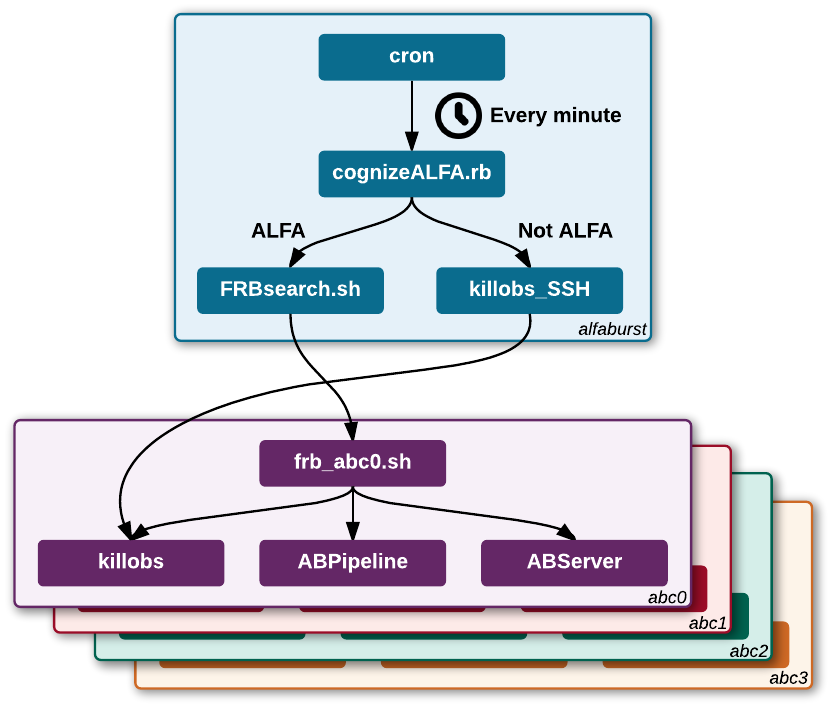
\includegraphics[width=0.6\textwidth]{abrunstop.png}
\end{center}
\caption{The cron job runs \protect\url{cognizeALFA.rb} every minute, which
checks if ALFA is the receiver in use. If yes,
\protect\url{FRBsearch.sh} is run. This script runs \protect\url{frb_abcX.sh}
on the compute nodes, where \protect\url{X} is the node identifier.
\protect\url{frb_abcX.sh} kills any existing processes using
\protect\url{killobs}, then runs both \protect\url{ABPipeline} and
\protect\url{ABServer}. When \protect\url{cognizeALFA.rb} discovers that ALFA
is no longer the receiver in use, it runs \protect\url{killobs_SSH}, which in
turn runs \protect\url{killobs} on the compute nodes, terminating data
acquisition.\label{fig_abrunstop}}
\end{figure}

Data acquisition relies on recognizing ALFA usage. This is achieved using a
cron job that invokes other scripts, as shown in Figure~\ref{fig_abrunstop}.


\subsection{Data Analysis}

Daily, manual monitoring of the generated plots is required. If an interesting
`blob' of data points is seen in a plot, the recommended procedure to follow is
given below.

We take as example, a plot generated on 7 September 2015, shown in
Figure~\ref{fig_dmvst}. This was a PALFA observing session, and as is typical
of such sessions, the observer observes a test pulsar first, in beam 0.
Ignoring the vertical streaks which are due to RFI, the test pulsar is the dark
blue (corresponding to beam 0) blob at a DM of about 100~cm$^{-3}$~pc near the
beginning of the observation. Towards the end of the observation, a set of
events is detected in beam 6 (red points), then in beam 5 (orange points), both
at a DM of about 250~cm$^{-3}$~pc. As we will see at the end of the following
steps, these sets of events are two single pulses of PSR B2002+31 when it
happened to be in the field of view, first in beam 6, and then in beam 5, as
the telescope slewed from one observing field to another\footnote{Although this
plot shows the power of the instrument in detecting transient events, it also
shows the difficulty involved in the manual inspection of plots, as there is no
quick way to differentiate between these two events and any of the RFI
events.}.

\begin{figure}[h]
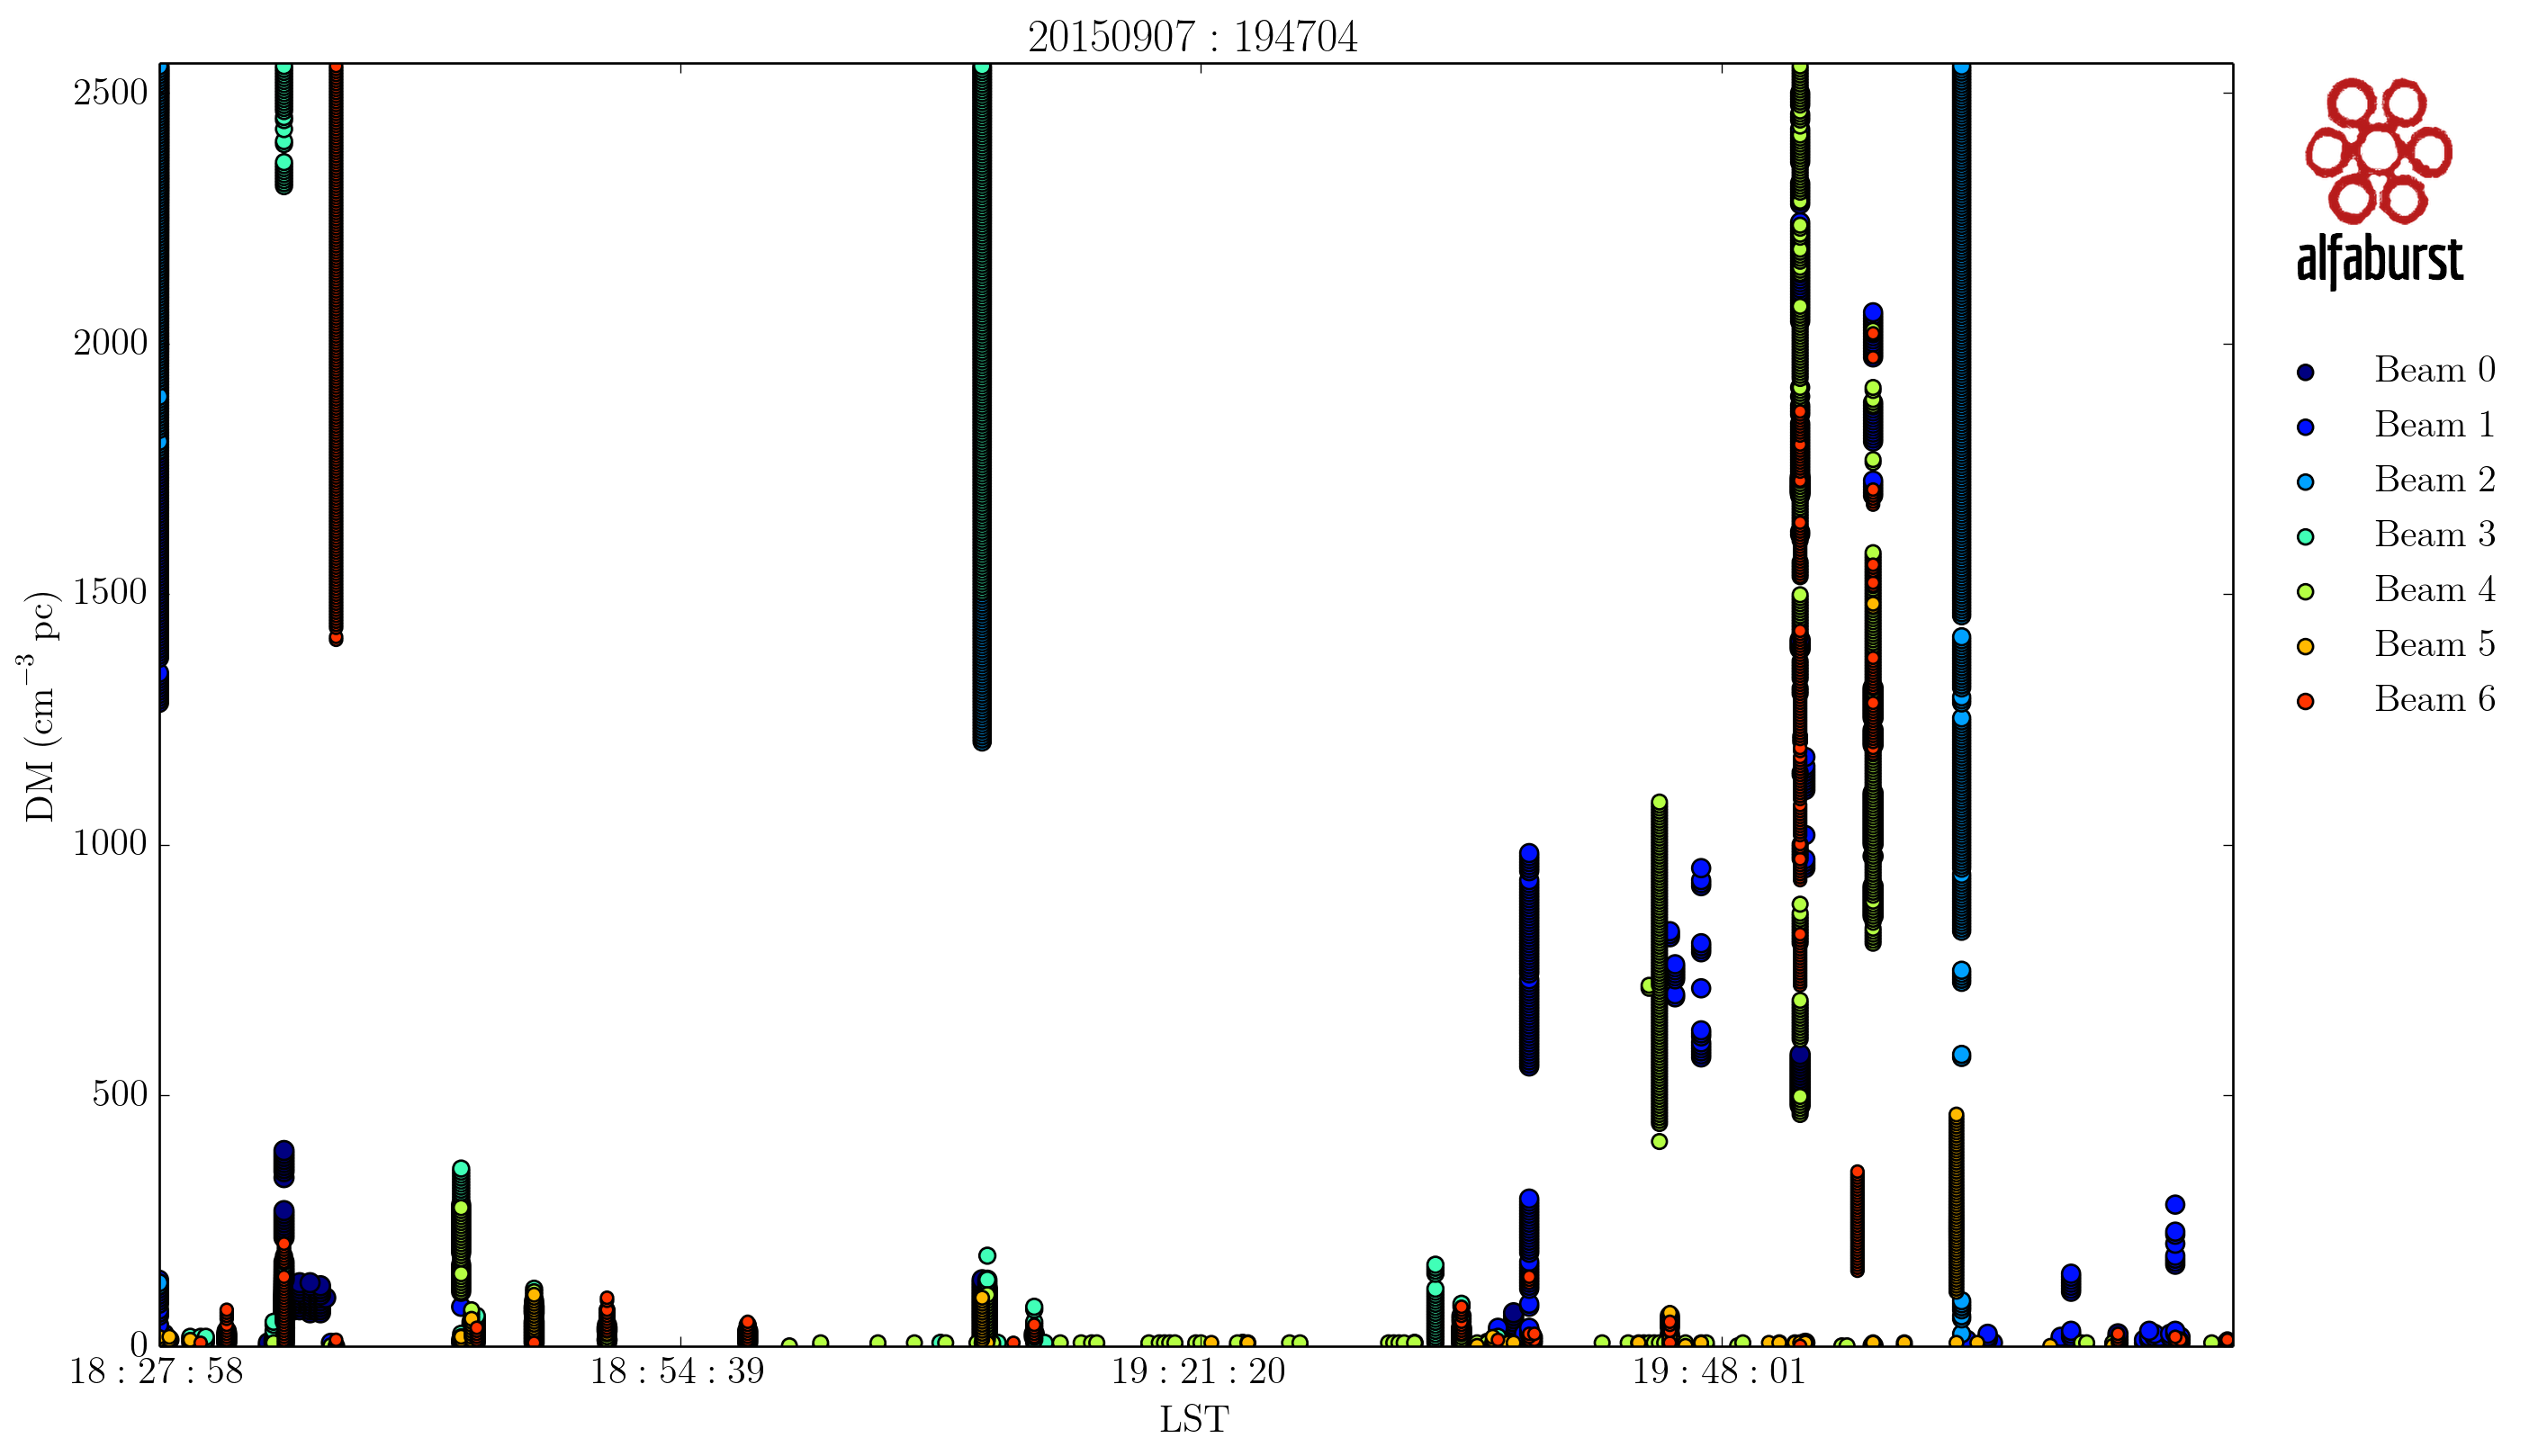
\includegraphics[width=\textwidth]{AllBeams_D20150907T194704.png}
\caption{Diagnostic plot with a test pulsar in beam 0 and PSR B2002+31 in beams
    6 and 5.\label{fig_dmvst}}
\end{figure}

\subsubsection*{Step 1: Get the buffer number}

First, check the \url{*dm*} file corresponding to the plot. SSH to \url{abc3},
corresponding to beam 6, and grep for the string `buffer' in the DM file.

\small{
\begin{verbatim}
$ grep buffer /data/Survey/Data/Beam6_dm_D20150907T194703.dat
...
# Written buffer :22 | MJDstart: 57273.04541088 | Best DM: 45 | Max SNR: 10.731744766235  Done
# Written buffer :23 | MJDstart: 57273.050023148 | Best DM: 1258 | Max SNR: 10.81814289093  Done
# Written buffer :24 | MJDstart: 57273.051967593 | Best DM: 262 | Max SNR: 13.327059745789  Done
# Written buffer :25 | MJDstart: 57273.052517361 | Best DM: 1227 | Max SNR: 10.498366355896  Done
# Written buffer :26 | MJDstart: 57273.06119213 | Best DM: 18 | Max SNR: 11.859872817993  Done
...
\end{verbatim}
}

We see that the best DM corresponding to buffer 24 matches what we see in the
plot. Examining this file in a text editor lets us see that the following is
the highest S/N event:

\small{
\begin{verbatim}
...
57273.052018887,   262, 13.327059745789, 32
...
\end{verbatim}
}

The event corresponds to a smoothing length of 32, which, at a sampling
interval of 256~$\mu$s, corresponds to a pulse width of 8.192~ms.


\subsubsection*{Step 2: Extract the buffer}

The filterbank file \url{} contains all the buffers in which events were
detected in this observing session, so we will extract just the buffer we are
interested in.

\small{
\begin{verbatim}
$ cd /data/Survey/Tmp
$ /home/artemis/Survey/Scripts/extractBuffer.rb -b 24 ../Data/Beam6_fb_D20150907T194703.fil
...
$ ls -ltrh
...
-rw-rw-r-- 1 artemis artemis 65M Jun  2 14:04 Beam6_fb_D20150907T194703.buffer24.fil
\end{verbatim}
}

As shown, we first move to a scratch area (\url{/data/Survey/Tmp}), so as not
to pollute the \url{/data/Survey/Data}) directory with temporary files. The
extracted filterbank file contains continuous time samples that can be analysed
like a standard filterbank file. The nodes have both
SIGPROC\footnote{\url{http://sigproc.sourceforge.net/}} and
YAPP\footnote{\url{http://jayanthc.github.io/yapp/}} installed for this purpose.

\subsubsection*{Step 3: Decimate the data}

Since the highest S/N event has a smoothing length of 32, we will decimate the
data in time, using SIGPROC (note that the output file size changes, as
expected).

\small{
\begin{verbatim}
$ decimate Beam6_fb_D20150907T194703.buffer24.fil -c 1 -t 32 > temp.fil
...
$ ls -ltrh
...
-rw-rw-r-- 1 artemis artemis 2.1M Jun  2 17:46 temp.fil
\end{verbatim}
}


\subsubsection*{Step 4: Plot the buffer}

We will use YAPP to visualise the data. First, we will dedisperse the buffer
visually, as shown below:

\small{
\begin{verbatim}
$ yapp_dedisperse -d 262 -m hot -g -n 1024 temp.fil
\end{verbatim}
}

\begin{figure}[h]
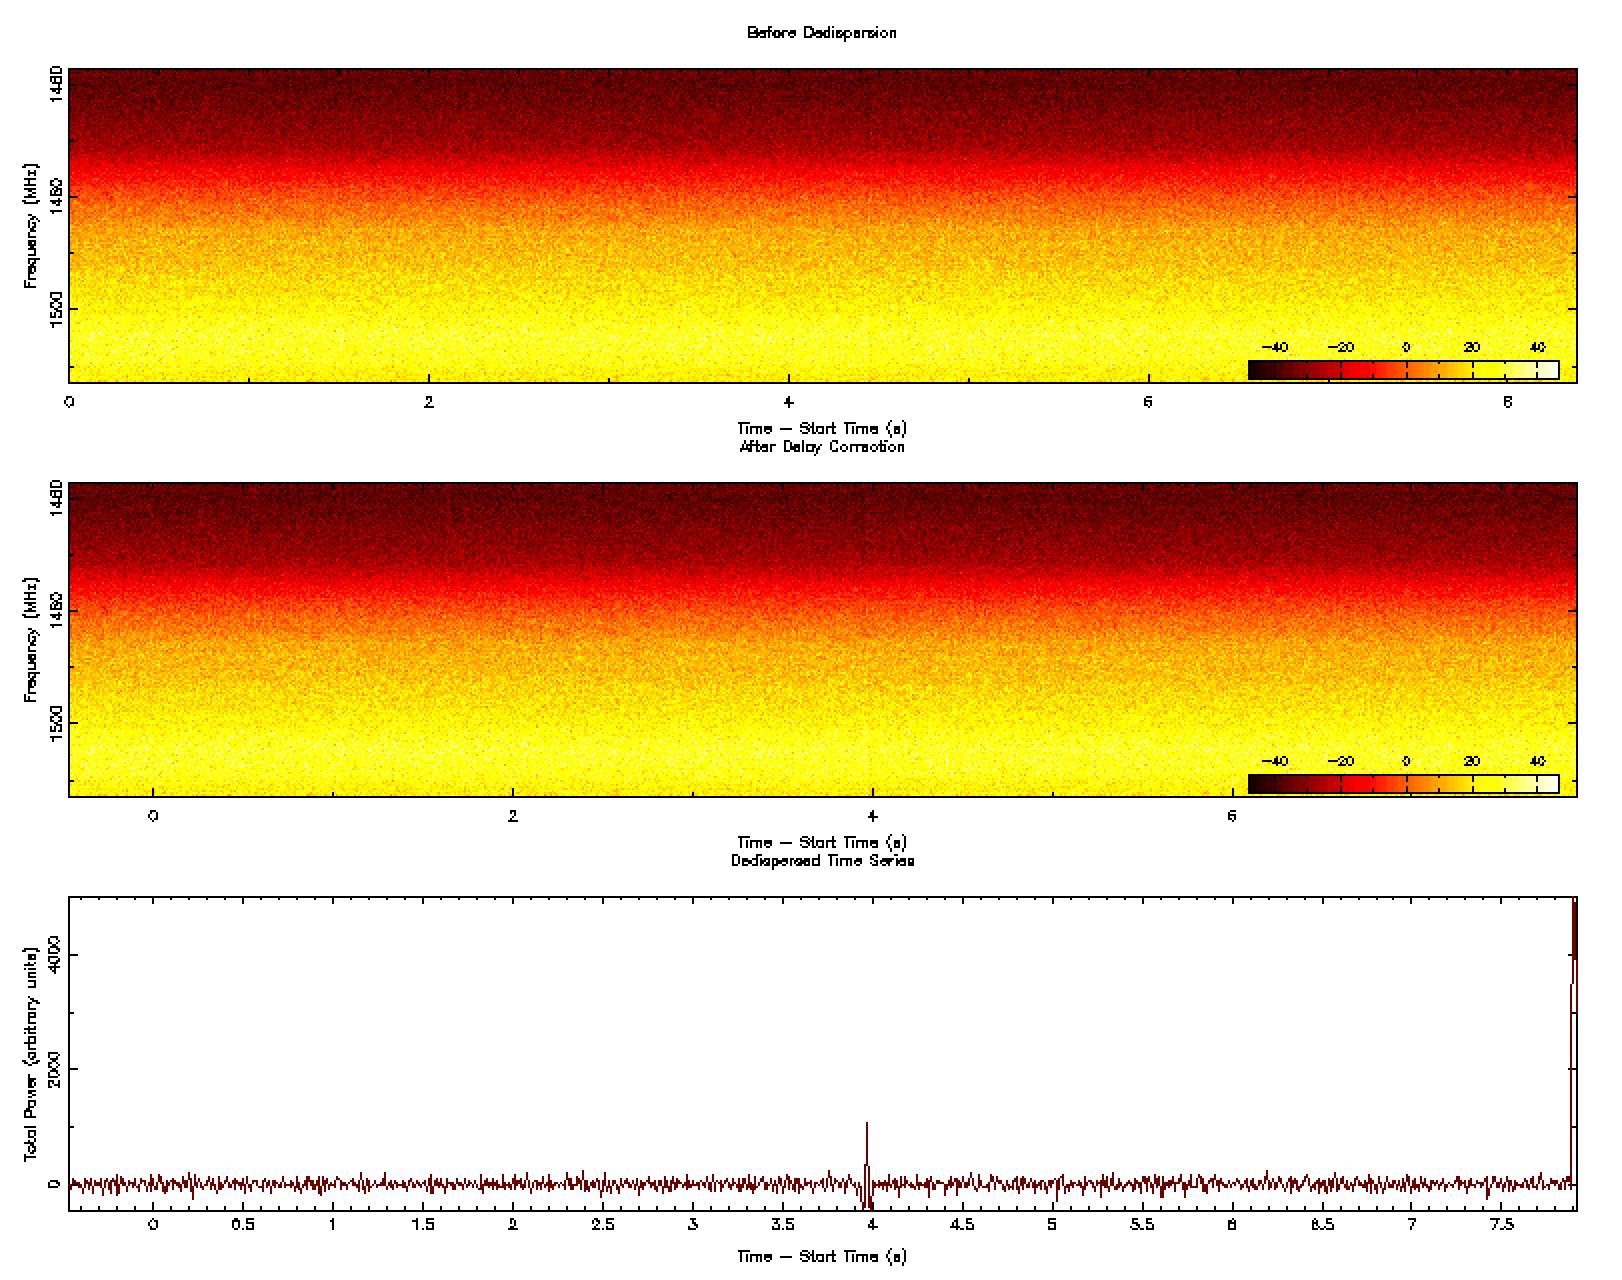
\includegraphics[width=\textwidth]{dd_tsnofs.png}
\caption{Data smoothed/decimated in time by a factor of 32, and dedispersed.
    A pulse can be seen between the 4- and 5-second marks in the dedispersed
    time series.
    \label{fig_dd_tsnofs}}
\end{figure}

Figure~\ref{fig_dd_tsnofs} shows the output of the above command, with the
pulse clearly visible in the dedispersed time series. Once we have confirmed
that there is clearly something in the dedispersed data, it is worth taking a
look at the filterbank data.

\small{
\begin{verbatim}
$ yapp_viewdata -m hot -n 1024 temp.fil
\end{verbatim}
}

\begin{figure}[h]
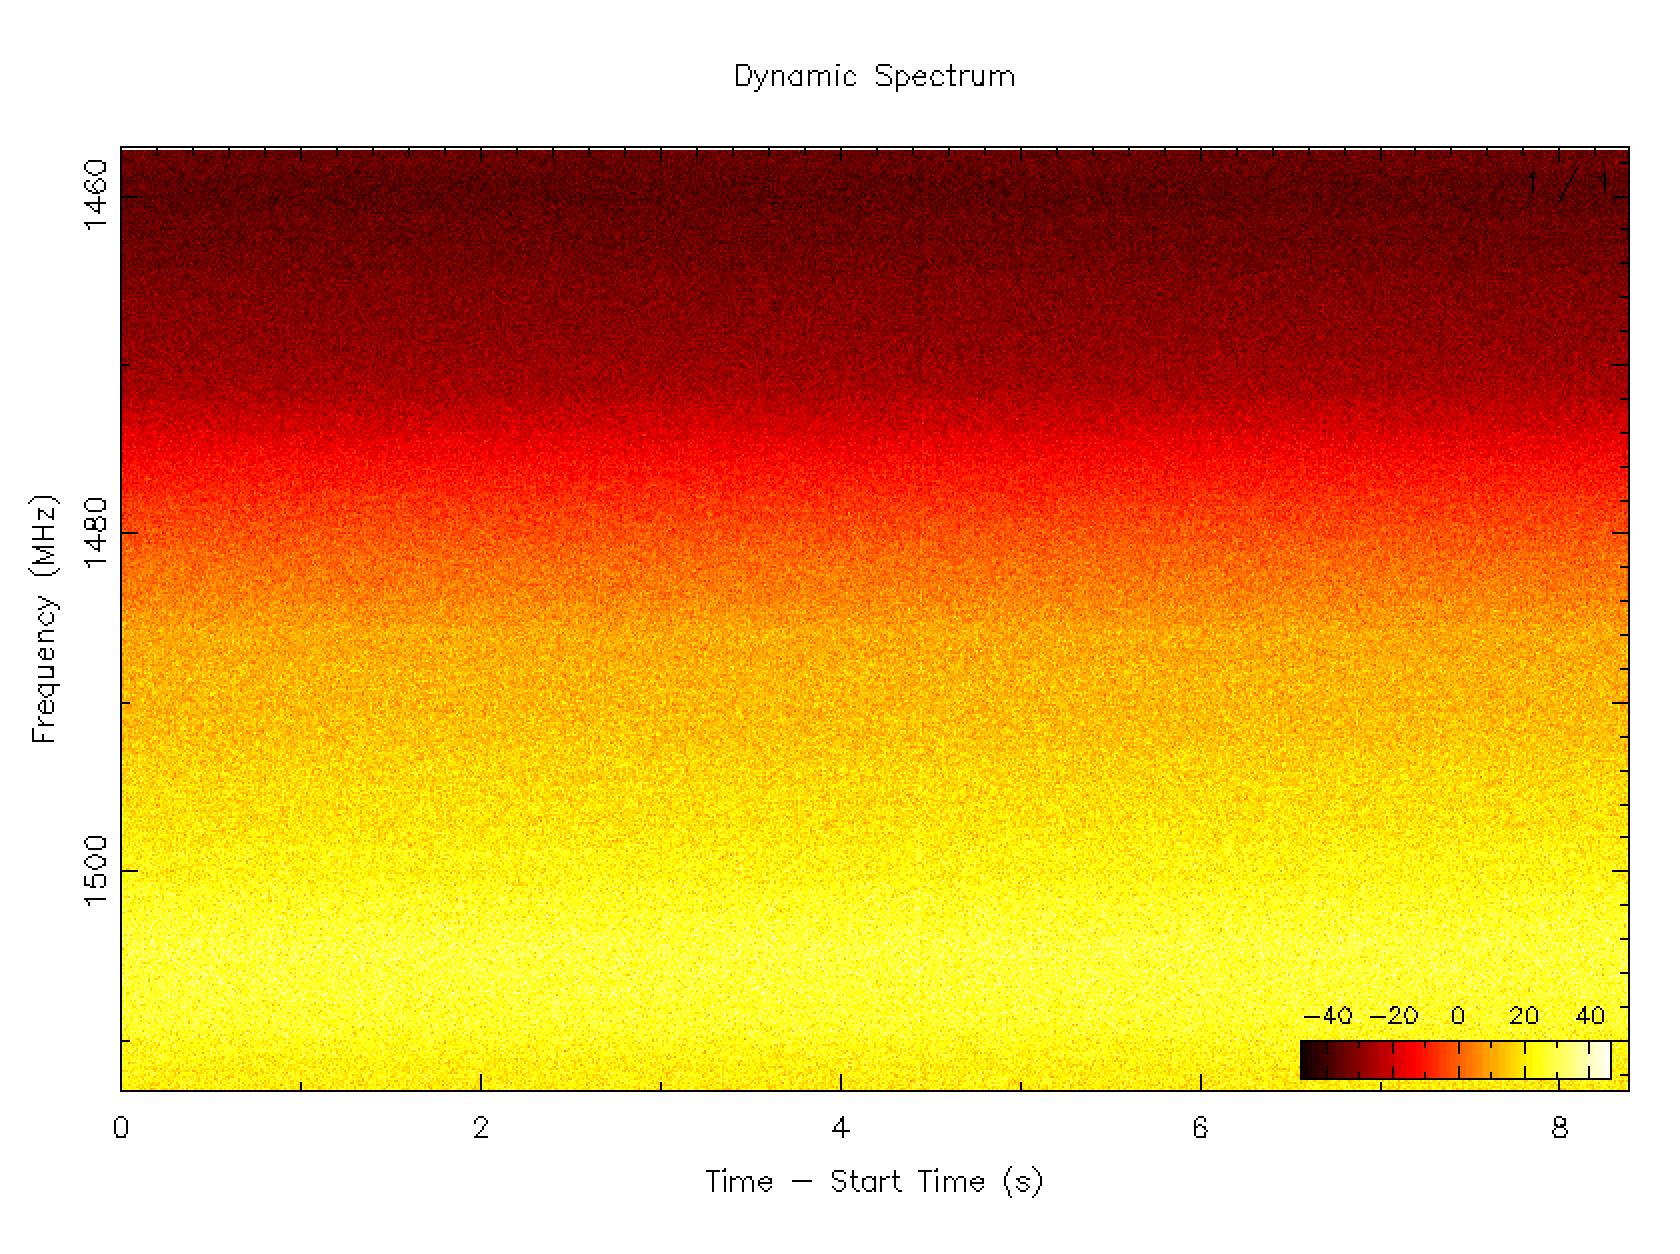
\includegraphics[width=\textwidth]{fb_tsnofs.png}
\caption{Data smoothed/decimated in time by a factor of 32. A pulse can be made
    out between the 4- and 5-second marks.
    \label{fig_fb_tsnofs}}
\end{figure}

As you can see in the output in Figure~\ref{fig_fb_tsnofs}, the dispersed pulse
can be just about made out, between the 4- and 5-second marks. If the plot is
zoomed in (for instance, by skipping the first 4 seconds, and processing only 1
second of data), the pulse becomes clearer, as shown in
Figure~\ref{fig_fb_tsnofs_zoomed}.

\small{
\begin{verbatim}
$ yapp_viewdata -m hot -n 1024 -s 4 -p 1 temp.fil
\end{verbatim}
}

\begin{figure}[h]
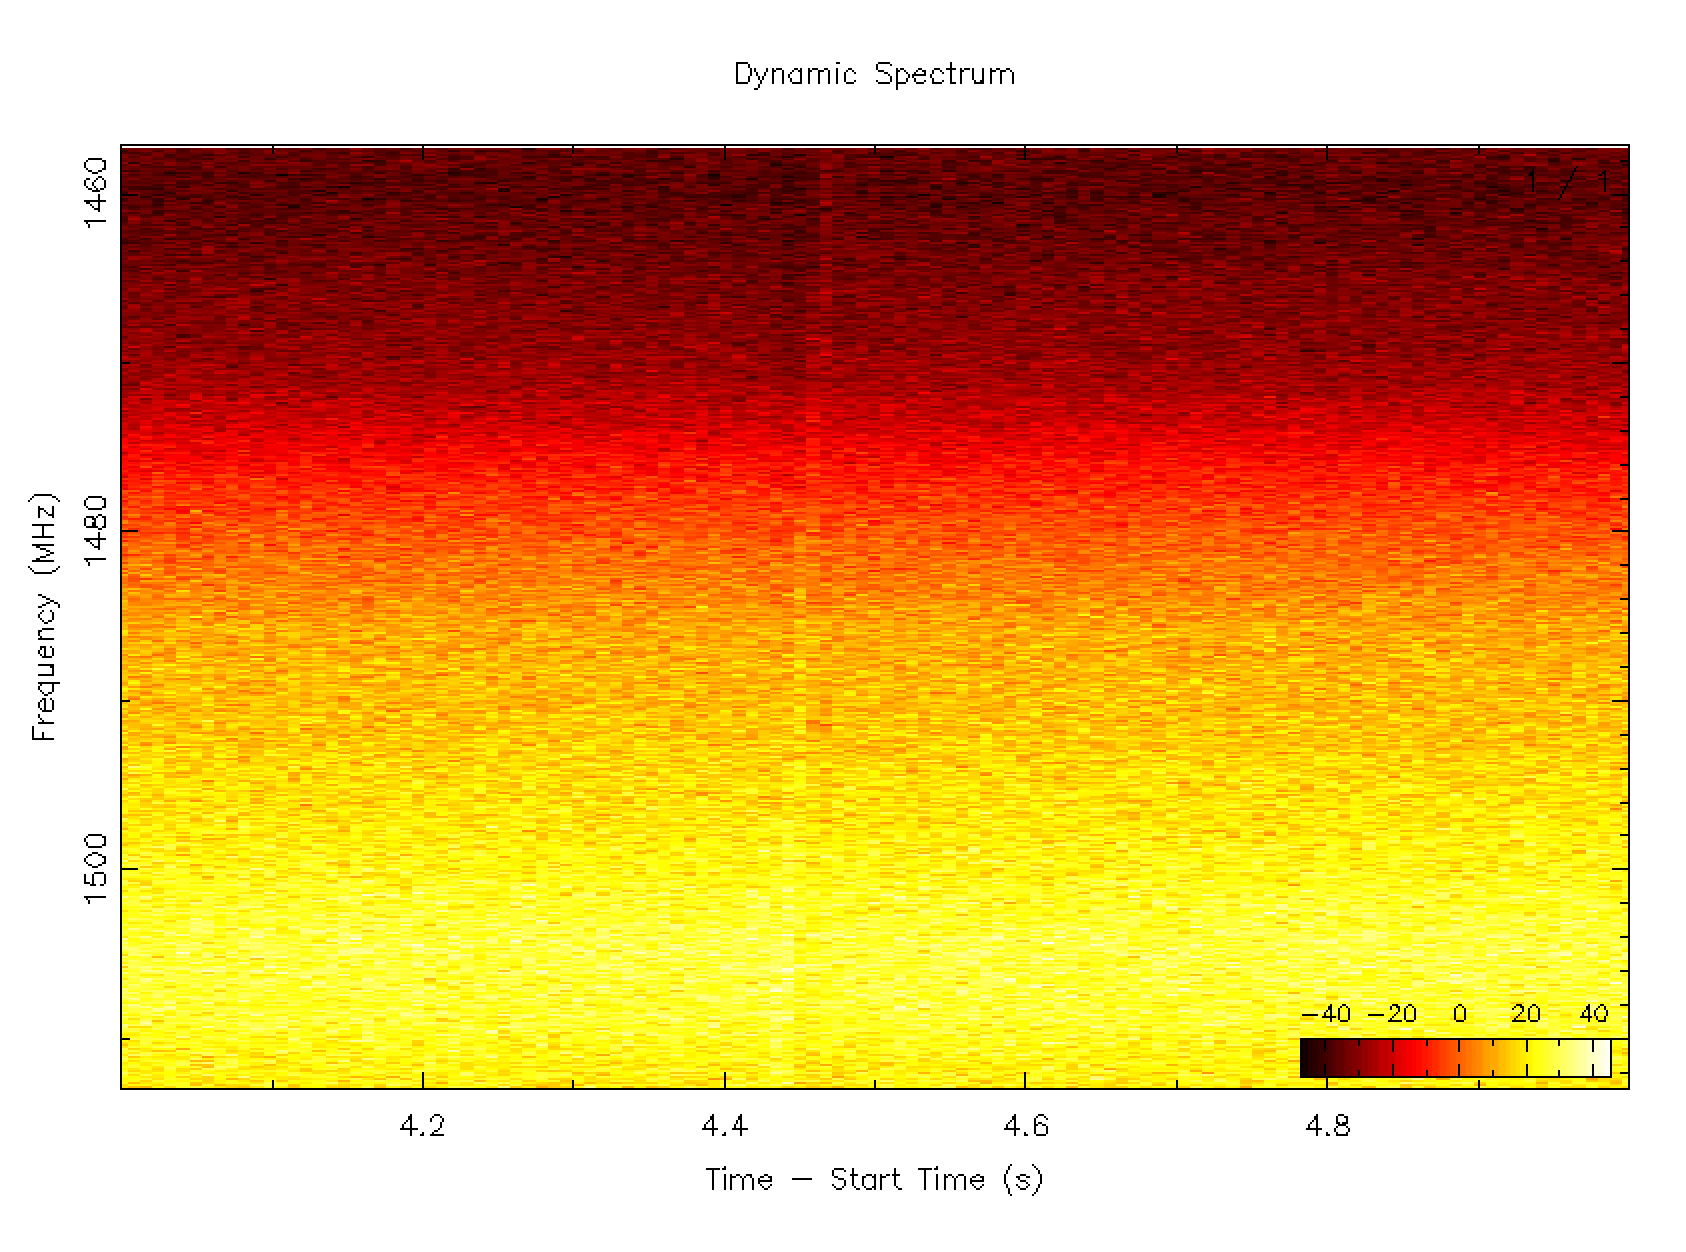
\includegraphics[width=\textwidth]{fb_tsnofs_zoomed.png}
\caption{Same as in Figure~\ref{fig_fb_tsnofs}, but zoomed in.
    \label{fig_fb_tsnofs_zoomed}}
\end{figure}

In Figure~\ref{fig_fb_tsnofs_zoomed}, the dispersed pulse can be clearly seen.
Note that, in some cases, the data may need to be decimated in frequency as
well, for the pulse to become apparent.

Note that, in addition to the $S/N$ of the pulse, rendering issues may affect
whether a pulse is apparent in the grayscale plots produced by YAPP, so it is
recommended that the dedispersion step above is also performed.

\textbf{Extracting the buffer may be optional:} Extracting the buffer is
required if one needs to proceed with decimating the data or do any other kind
of signal processing. However, if one is interested only in viewing the raw
data, YAPP can be used as follows. Since we know that each buffer is
32768~samples long and each sample represents 256~$\mu$s, we can just skip the
duration corresponding to 23 buffers' worth of data (note that buffer counts
start at 1).

\small{
\begin{verbatim}
$ yapp_viewdata -m hot -n 32768 -s 192.937984 ../Data/Beam6_fb_D20150907T194703.fil
\end{verbatim}
}

\subsubsection*{Step 5: Get pointing information}

Once we have visually confirmed that a real pulse exists in our data, it is
time to check if it originated in any of the known sources. The first step in
this process is to get the pointing of the beam that the pulse was found in. To
do this, we need to use the raw SCRAM dump for the day of the observation,
resident on the S6 head node, in \url{/data/serendip6}. The script
\url{/home/artemis/getPointings.rb} on \url{serendip6} copies the SCRAM dump to
a scratch area and extracts the pointing information, given the MJD of the
event (found in the \url{*dm*} file).

\small{
\begin{verbatim}
$ /home/artemis/getPointings.rb -m 57273.052018887 -u
1441674894
ls /data/serendip6/scramdump.* | cut -d '.' -f 2
/data/serendip6/scramdump.1441728353.gz.at_ucb
cp -a /data/serendip6/scramdump.1441728353.gz.at_ucb /home/artemis/
gunzip --force --name --suffix '' /home/artemis/scramdump.1441728353.gz.at_ucb
s6_observatory -nodb -stdout -infile /home/artemis/scramdump.1441728353 2>&1 > /dev/null ...
... | grep 1441674894 | sort | uniq | grep RA0 | tail -1
SCRAM:DERIVED DERTIME 1441674894 RA0 20.0870184820 DEC0 31.6797526839 RA1 ...
20.0882034790 DEC1 31.5762092232 RA2 20.0937621054 DEC2 31.6480614290 RA3 ...
20.0925845567 DEC3 31.7517543100 RA4 20.0858295333 DEC4 31.7832084015 RA5 ...
20.0802614126 DEC5 31.7107828505 RA6 20.0814576722 DEC6 31.6074755720
rm -f /home/artemis/scramdump.1441728353
\end{verbatim}
}

The above script can also be run from the AB machines (as opposed to logging on
to \url{serendip6}), as follows:

\small{
\begin{verbatim}
$ ssh artemis@serendip6 "/home/artemis/getPointings.rb -m 57273.051967593 -u"
...
\end{verbatim}
}

Note that this takes around 20 minutes to run.


\subsubsection*{Step 6: Plot the beam pointings}

The next step is to plot the pointings obtained from the SCRAM dump, along with
the positions of all known pulsars in the vicinity of the beams on the sky. We
will use \url{/home/artemis/Survey/Scripts/alfabeams.py} on \url{alfaburst} for
this. First, copy the RA and declination information output by
\url{getPointings.rb} into a file named \url{pointings}, in the following
format:

\small{
\begin{verbatim}
RA0,DEC0
RA1,DEC1
RA2,DEC2
RA3,DEC3
RA4,DEC4
RA5,DEC5
RA6,DEC6
\end{verbatim}
}

Create a file named \url{sources} with the RA and declination information of
all known sources that you would like to plot, in the same format as above.
(NOTE: \url{alfabeams.py} needs to be edited a little to do this part.) Then
run the script. Figure~\ref{fig_pointings} shows a sample plot, where PSR
B2002+31 is plotted along with all beam pointings when a pulse from that source
was detected in beam 6 (see the diagnostic plot in Figure~\ref{fig_dmvst}). It
is now clear that the event seen in the diagnostic plot is a known pulsar. For
the discovery of a new source, such a coincidence should not be present.

\begin{figure}[h]
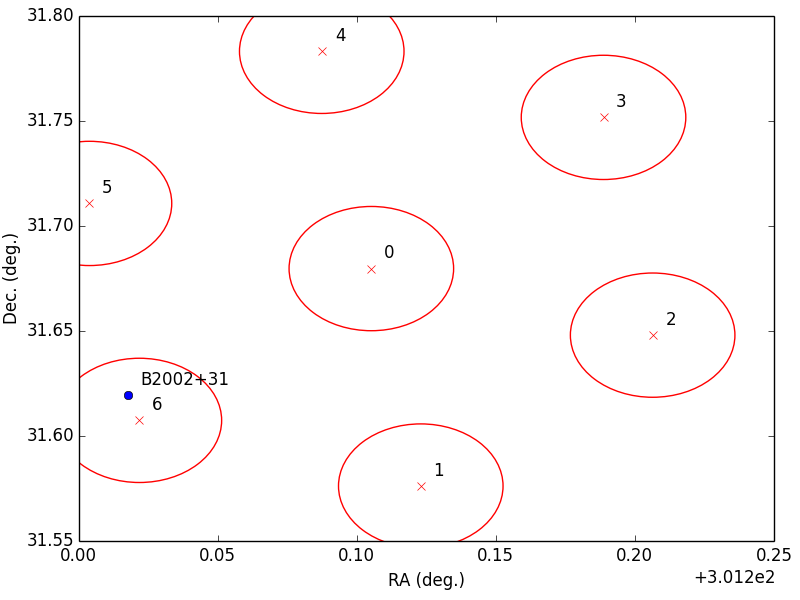
\includegraphics[width=\textwidth]{pointings.png}
\caption{Plot of all beam pointings, showing the coincidence of beam 6 with the
location of PSR B2002+31.\label{fig_pointings}}
\end{figure}


\section{Miscellaneous Notes}

\subsection{Power Control}

IPMI is used for node management independent of the OS. Among other things, it
can be used to check if the power to a node is on, power on and off a node, and
use Serial-Over-LAN to watch the remote system boot and access its terminal.
The following are the power commands, where \url{N} is the node identifier (0,
1, 2, or 3). The \url{x} appended to the node name indicates the IPMI
interface.

\small {
\begin{verbatim}
$ ipmitool -I lanplus -U ADMIN -P ADMIN -H abcNx power status
$ ipmitool -I lanplus -U ADMIN -P ADMIN -H abcNx power on
$ ipmitool -I lanplus -U ADMIN -P ADMIN -H abcNx power off
\end{verbatim}
}

To activate Serial-Over-LAN (to see system messages as it boots, for example),
the following command is used.

\small {
\begin{verbatim}
$ ipmitool -I lanplus -U ADMIN -P ADMIN -H abcNx sol activate
\end{verbatim}
}


\subsection{Bad Node}

The compute node \url{abc2} goes offline sometimes. Power seems to be on
according to IPMI, but the machine is unreachable over the network. When this
happens, power cycle the node over IPMI.


%\subsection{Logging}

%Multiple log files are generated/appended to during AB observations.


\end{document}

